\chapter{Introduction}

\begin{mynote}
\subsubsection{Chapter outline}
In this chapter, I outline the problem I am addressing in this thesis, and the proposed contribution.
\end{mynote}

\vspace{10pt}

\section{Motivation}
Imagine, you have come back from a business trip and have to claim back your expenses. You open the expenses system and enter the first few personal details such as your name from the top of your head without any problem. For the expenses you want to claim back, you get up to collect your receipts from your wallet and start entering the items and prices into the system. The prices are in a foreign currency, so you leave the expenses system to go to a currency converter website and convert the prices. You then need to enter your account number. You go and get your wallet with bank cards from your bag. How many times have you stopped entering to go and look up certain information? Or did you get all the required information beforehand, so you did not have to get up in-between? You may have entered the information you knew first, and left the remaining items until the end? Whatever way you chose to complete the task, it involved making decisions on how to manage subtasks of looking up the required information for the entry task. 

Data entry is usually a straightforward task, but when information has to be retrieved from multiple sources, not all of which are as easy to access, this simple task can quickly become complex. Interrupting a data entry task to look up the required data can be disruptive, as you have to pay a time cost 
each time you resume your data entry task. You may have forgotten where you were, enter information in the wrong place, or misremember what you were supposed to enter and enter something incorrect. This disruption can introduce data entry errors, the outcomes of which can range from annoying to more serious consequences, such as transferring money to the wrong bank account, or transferring a wrong amount.  

Because it is important data entry is done accurately, data entry research has looked at improving the input interfaces \citep[e.g.][]{Oladimeji2013, Vertanen2015, Wiseman2013a}, but it is not clear its design implications generalise to the type of situation as described above. In this situation, you do not enter all items from a source nearby, as in most data entry studies, but need to retrieve and enter different types of information (e.g. numbers, alphanumeric strings, words) from multiple sources (e.g. e-mails, paper receipts, different computer windows). The time cost to access these resources varies, and if information becomes harder to access, people increasingly rely on what they have memorised of the information rather than recheck the resource \citep{Gray2006}. It is however not known how people prioritise and manage their tasks when they have to retrieve the information from multiple resources, with varying access costs, or how a data entry interface should be designed to support people in these situations. 

While it has been shown how changing the design of a data entry interface can affect and improve how we enter data, and that different information access costs affect how often people consult one source, it is not known how the interface can support situations when data has to be retrieved and entered from various sources with varying information access costs. In order to design interactive systems that truly support this type of data entry task, it is necessary to get a detailed understanding of how users manage this task and its subtasks, and to what extent the access to the required resources affect their strategies.

This thesis investigates how different time costs affect how people manage self-interruptions to look up information for a data entry task, with the aim to inform the design of data entry systems. 
%In order to design systems that truly support the task they are intended for, it is necessary to get a detailed understanding of this task. 

For the scope of this thesis, I look specifically at how employees in financial administration offices manage self-interruptions to look up information for an expenses task. This task requires entering different types of information from a variety of sources, such as paper, spreadsheets, emails and databases. It is important the task is done accurately but within a reasonable amount of time as they are under time pressure to finish work on time. This data entry task is therefore considered to be an appropriate and interesting example to study further. 

The expenses task serves as an example of a wider class of data entry tasks, and it can be imagined findings of this thesis can be useful and generalise to other, similar, tasks. For example, people who have to fill in their tax returns have to similarly enter a range of information into a computer system, and have to collect this information from multiple sources with varying IACs.

The research question of this thesis is:

\textbf{How can time costs be used to support interruption management of inquiries for a routine data entry task?}

This research question is addressed by answering the following subquestions which are addressed in different chapters:

\begin{enumerate}
\item How do people manage inquiries for data entry in a finance office setting? (Chapter 3)
\item What is the effect of time costs on the number, duration and timing of inquiries for a data entry task?  (Chapter 4)
\item  Does time feedback affect the number and duration of inquiries for data entry? (Chapter 6)
\end{enumerate}

%\begin{enumerate}
%\item Does the IAC of information sources affect how people manage subtasks to look up information for an expenses task in a finance office setting?
%\begin{enumerate}
%\item	What (types of) information do people need for entering expenses?
%\item	Where do people need information from?
%\item	How do they address those needs?
%\item	Does the type of information, and where they need it from, affect how people address these needs?
%\end{enumerate}
%\item	How can the existing data entry system be redesigned to support or better support people managing subtasks of looking up information for entering expenses, given variable IACs for required information sources?
%\end{enumerate}

\section{Thesis outline}
Chapter 2 discusses related literature. It first discusses prior research on interruptions at the workplace, on information seeking and management, and technology interventions to address interruptions and information management. It also gives an overview of prior data entry research. This literature review highlights that it is important to get a detailed understanding of data entry work in its situated context, in order to support people in managing inquiries during data entry. 

Chapter 3-6 describe seven studies conducted to address the research question of this thesis. Chapter 3 describes two qualitative studies aimed to get a detailed understanding of data entry work in a finance office setting. These studies revealed that a major part of data entry is retrieving information from multiple sources with varying time costs. Chapter 4 reports three laboratory experiments to test the hypothesis that time costs influence the number, duration and timing of inquiries for a data entry task. These studies showed that people postpone interruptions with high time costs. Chapter 5 explores different design ideas, based on the research findings so far and prior literature. It describes the development and design of a browser notification which is based on the premise that showing time costs to users may help people manage interruptions outside a controlled setting. Chapter 6 describes an online experiment and a field study to evaluate the effectiveness of this browser notification showing the time costs of interruptions during data entry work. These studies showed that making people more aware of time costs can act as a trigger to reflect on what they were doing during prior interruptions, and encourages them to shorten their interruptions.

Chapter 7 summarises the key findings of the studies. It discusses the contribution that these findings make to knowledge and what the practical implications are. It also discusses opportunities for future work. 

The thesis structure is depicted as a diagram in Figure \ref{fig:ch1-thesisoverview}.


\begin{figure}
\centering
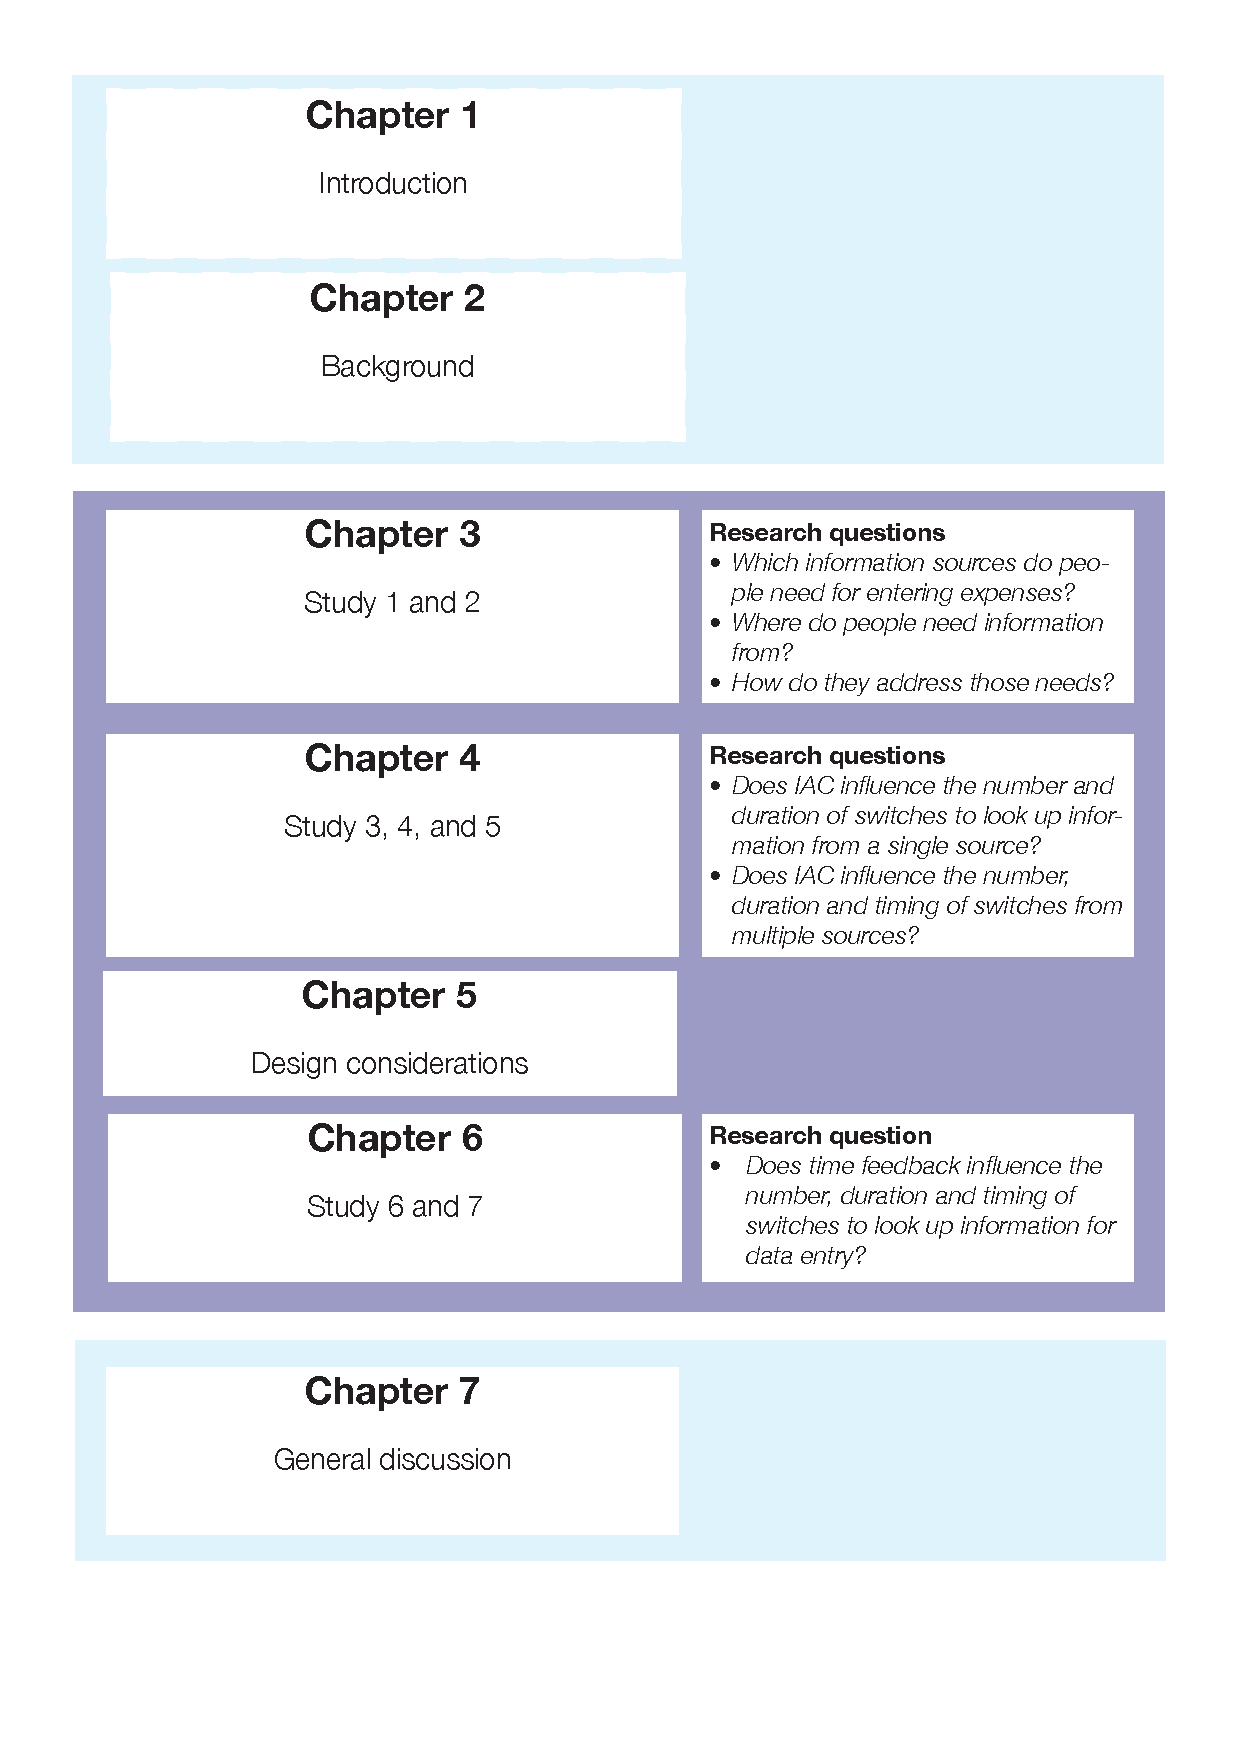
\includegraphics[width=1\textwidth]{images/ThesisOverview.pdf}
\caption{Visual overview of the thesis structure.}
%\vspace{-3pt}
\label{fig:ch1-thesisoverview}
\end{figure}

\section{Contribution}
The first contribution of this thesis is to map out the fragmented nature of an expenses task, of which looking up information is a substantial part of the task. It investigates how the time cost of accessing required information sources affects how people manage when they look up certain information. This finding has implications for the design of the current system: a second contribution is demonstrating how changing certain design features can better support people in managing these subtasks of looking up information.
